\section{Preliminaries}
\label{sub_pre}
In this section, we first provide a formal definition of the table union search task, and then introduce the overview of the main components in our framework. 

A table is a collection of several columns $\{c_1,\dots,c_n\}$, where each column $c_i$ can be from different domains. For simplification, we use $t$ to denote both the table and its set of columns if there is no ambiguity. 

\noindent\textit{Task Definition.} Given a query table $q$ and a table corpus $\mathcal{T}$, let $U(q,t)$ denote the $t$'s unionability degree to query table $q$. The purpose of table union search aims to return a list top-$k$ tables $\{t_1,\dots,t_k\}$ from $\mathcal{T}$, which satisfies $\forall t\in\{t_1,\dots,t_k\}$ and $\forall t'\in\mathcal{T}\backslash \{t_1,\dots,t_k\}$, $U(q,t)\geq U(q,t')$. 

%For the unionability $U(q,t)$, it measures how much all the columns in $q$ can be unioned with an existed column in $T$. Hence, we define the column relevance score $\mathcal{S}(\cdot,\cdot)$, which are always calculated by the embeddings of columns, i.e., for column $q_i\in q$ and $t^j\in T$, $\mathcal{S}(\mathcal{E}(q_i),\mathcal{E}(t^j))$ is the relevance score between column $q^i$ and $t^j$, where $\mathcal{E}(\cdot)$ is a column/table encoder function. Besides, we define a function $\mathcal{A}$ to aggregate the column relevance scores between all pairs of columns from the two tables. 

\begin{figure*}
    \centering
    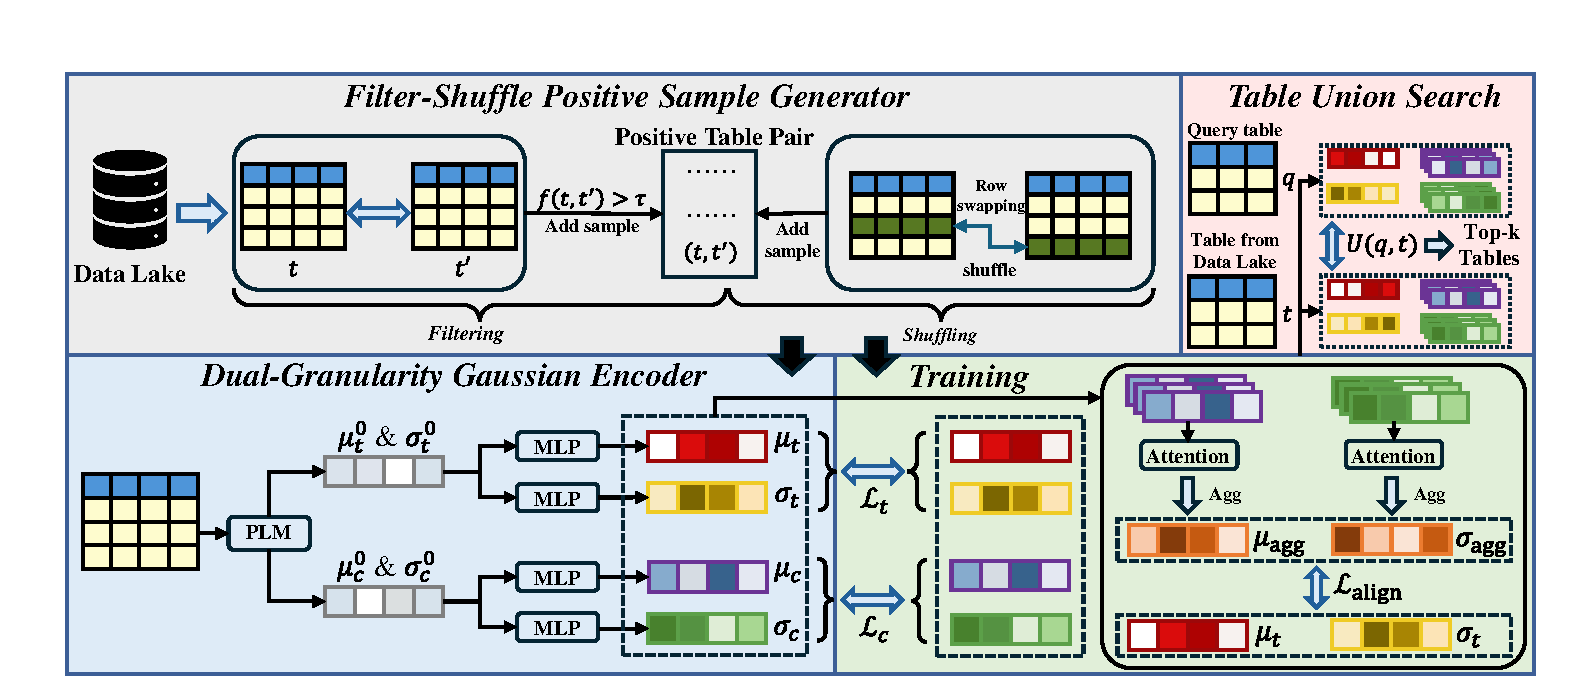
\includegraphics[width=\textwidth]{figure/overview.pdf}
    \caption{
        \textbf{The framework of DGGC.} 
    }
    \label{fig:over}
\end{figure*}

\section{Preliminaries}
\label{sub_pre}

We first formalize the table union search task and introduce the main notations used in DGGC.

A table $t$ consists of a set of columns $\{c_1, \dots, c_n\}$, where each column may belong to a distinct semantic domain. When no ambiguity arises, we use $t$ to denote both the table and its column set.

\noindent\textit{Task Definition.} 
Given a query table $q$ and a corpus $\mathcal{T}$, let $U(q,t)$ denote the unionability score between $q$ and a candidate table $t$. The objective of table union search is to retrieve the top-$k$ tables $\{t_1,\dots,t_k\} \subset \mathcal{T}$ such that
\[
\forall t \in \{t_1,\dots,t_k\},\ \forall t' \in \mathcal{T}\setminus\{t_1,\dots,t_k\},\quad
U(q,t) \ge U(q,t').
\]

Figure~\ref{fig:over} illustrates the overall framework of DGGC.
